%!TEX root = these.tex

\chapter[Analyse de l'acquisition de cibles mobiles]{Analyse de l'acquisition de cibles mobiles}
\minitoc
\label{chap4}
\cleardoublepage

\section{Introduction}
	Dans ce chapitre nous présentons les résultats d'une étude empirique visant à caractériser les performances de sélection de cibles mobiles en fonction de la nature de leurs mouvements, dans un contexte aussi simple que possible : un ordinateur de bureau avec un écran monoscopique et une souris. Notre objectif étant de mieux comprendre cette tâche, dans le but éventuel d'aboutir à un modèle fiable, nous avons en effet cherché à limiter autant que possible l'influence de facteurs tels que la stéréoscopie (éventuellement adaptative), la nécessité de déplacements du corps entier, l'utilisation de périphériques peu familiers, etc. 
	
	Nous revenons premièrement sur le modèle de génération de mouvement introduit dans le chapitre~\ref{chap3}, ses capacités et limitations, et son extension 3D. Nous proposons d'autres extensions de ce modèle permettant de gérer les cas actuellement hors de sa portée.
	
	Nous étudions ensuite l'effet individuel des paramètres d'angle, de fréquence et de vitesse issus de notre modèle, puis les interactions entre ces effets. Nous relions ces paramètres et les conditions qu'ils engendrent aux impressions subjectives des participants à notre étude, afin d'établir quels facteurs perceptifs ou cognitifs influent sur les performances de sélection, selon la nature du mouvement des cibles.

	Dans ce but, nous examinons d'une part les profils de vitesse du curseur lors des tâches de sélection, en mesurant la durée relative de la phase balistique, et d'autre part le pouvoir prédictif des enveloppes convexes, introduites dans le chapitre~\ref{chap3}.
	
	Sur la base des enseignements que nous en tirons, nous proposons un guide pour la conception de techniques de sélection spécifiquement orientées vers les cibles mobiles, en précisant comment la nature des mouvements influe sur les contraintes imposées par la tâche, et sur les solutions possibles.

\section{Génération de mouvements}
	Si notre objectif est de caractériser les performances de sélection pour des cibles mobiles en fonction de la nature de leurs mouvements, notre intérêt se porte plus particulièrement sur les cibles de mouvements \og erratiques \fg{}, \og imprévisibles \fg{}, ou rappelant ceux d'une mouche.
	
	Ce focus a principalement deux motifs : premièrement, les chercheurs spécialisés dans la biologie structurale tentant d'utiliser des techniques de simulation de dynamique moléculaire interactive (voir le chapitre~\ref{chap1}) nous ont exprimé leurs difficultés d'interaction avec leurs systèmes, et particulièrement de sélection. Deuxièmement, de rapides tests empiriques suggéraient que les mouvements de ce type causaient les plus grandes difficultés pour des tâches de sélection.
	
	\subsection{Modèle VFA}
	Afin de tester cette hypothèse, nous avons conçu un modèle de génération de mouvements permettant, à l'aide d'un nombre de paramètres aussi petit que possible, de générer des mouvements aussi variés que possible dans leur nature. Pour rappel, il s'agit du modèle évoqué dans le chapitre~\ref{chap3}, et décrit par les paramètres suivants, pour définir le mouvement d'un objet de vecteur direction $\vec{dir}$ :
	
    \begin{enumerate}
    	\item La vitesse $V$ à laquelle l'objet se déplace ;
    	\item La fréquence $F$ des changements de $\vec{dir}$ ;
    	\item L'angle maximal $A$ de ces changements de direction : à chaque période $T = \frac{1}{F}$, $\vec{dir}$ subit une rotation d'un angle $\alpha$ échantillonné uniformément dans l'intervalle $[-A, +A]$.
    \end{enumerate}
    
    Du fait de son fondement sur les paramètres $V$, $F$ et $A$, nous appellerons simplement ce modèle $VFA$.
    
    \subsection{VFA en 3D}
    Quelques observations s'imposent. Tout d'abord, bien que décrit ici pour deux dimensions, ce modèle est naturellement extensible à l'espace tridimensionnel. En effet, les paramètres $V$, $F$ et $A$ ne changent pas ; seule un ajustement est nécessaire : la rotation du vecteur direction de l'objet animé doit se faire selon un axe qui, pour que la rotation effective soit toujours la même pour un angle donné, doit être orthogonal à $\vec{dir}$. Notre modèle étendu VFA3D fonctionne donc comme le modèle VFA, mais avec un axe de rotation orthogonal à $\vec{dir}$ choisi aléatoirement.
    
    \subsection{Un modèle puissant mais limité}
	Les capacités offertes par le modèle VFA sont très nombreuses, mais demeurent limitées, et ne peuvent couvrir tous les besoins possible en matière de génération de mouvement aléatoire.
    
    \subsubsection{Vitesse constante}
    Comme nous l'avons partiellement montré dans le chapitre~\ref{chap3}, le fait de varier les paramètres, en particulier $F$ et $A$, permet de générer des types de mouvement subjectivement très différents (voir les figures~\ref{fig:motion1530}, \ref{fig:motion4560}, \ref{fig:motion7590}, \ref{fig:motion105120}, \ref{fig:motion135150} et \ref{fig:motion165180}), et d'enveloppes convexes de tailles très différentes également (voir la figure~\ref{fig:trajAreas}). Néanmoins, et outre le problème des objets autocorrélés, notre modèle repose notamment sur une vitesse constante, ce qui, de fait, exclut tous les objets susceptibles d'accélérer. Là encore, ce choix fut fait pour limiter le nombre de paramètres, toujours dans l'objectif d'atteindre un compromis entre la simplicité du modèle et sa capacité à générer des mouvements que nos sujets puissent percevoir comme fondamentalement différents.
    
	Nous souhaitions tout particulièrement pouvoir générer du mouvement perçu comme \og régulier \fg{} ou \og prévisible \fg{} ainsi que du mouvement \og irrégulier \fg{}, \og saccadé \fg{} ou \og imprévisible \fg{}.
    
   	\subsubsection{Pas de véritable autocorrélation}
	Une autre obsevation très importante est que ce modèle ne peut générer que du mouvement markovien. En effet, à l'instant $t+1$, la rotation de $\vec{dir}$ générée est totalement indépendante de celle éventuellement générée à $t$, ou plus généralement de la dernière rotation générée, si elle existe. Cela ne signifie pas que $\vec{dir}_{t+1}$ soit indépendant de $\vec{dir}_{t}$, et il ne l'est pas, mais que le changement de direction à tout instant est indépendant du passé de l'objet concerné.
    
    Il en résulte que ce modèle ne peut générer du mouvement permettant d'étudier les performances de sélection sur des objets autocorrélés, tels que nous les avons définis et énumérés au cours du chapitre~\ref{chap3}. Ce choix reflète d'une part notre focus originel sur les simulations moléculaires (où il y a une demande claire émanant des utilisateurs) et d'autre part une volonté de conserver un modèle aussi simple que possible, afin de le rendre plus facile à utiliser, mais aussi pour pouvoir évaluer un échantillon représentatif des types de mouvements qu'il peut générer dans un laps de temps raisonnable pour une étude empirique, compte tenu notamment de la fatigue des sujets.
    
    \subsubsection{Mouvements pseudo-autocorrélés}
	Remarquons tout de même qu'une trajectoire générée par notre modèle peut, au moins temporairement, approximer un mouvement autocorrélé. Attendu qu'une tâche de sélection, pour peu qu'elle ne soit pas trop difficile, peut se dérouler sur une durée inférieure ou égale à la durée pendant laquelle le modèle VFA peut approximer un mouvement autocorrélé, il n'est pas nécessairement inutile pour étudier les performances de sélection de ces objets. On privilégiera dans ce cas de très fortes valeurs de $F$ et de très faibles valeurs de $A$. La figure~\ref{fig:autocorr} fournit deux exemples de telles trajectoires que nous proposons d'appeler pseudo-autocorrélées, générées avec $F \in \{30,120\}$ et $A \in \{1,2\}$.
	
	\begin{figure}[!htb]
		%\centering
		\begin{subfigure}[t]{0.49\textwidth}
			\centering
			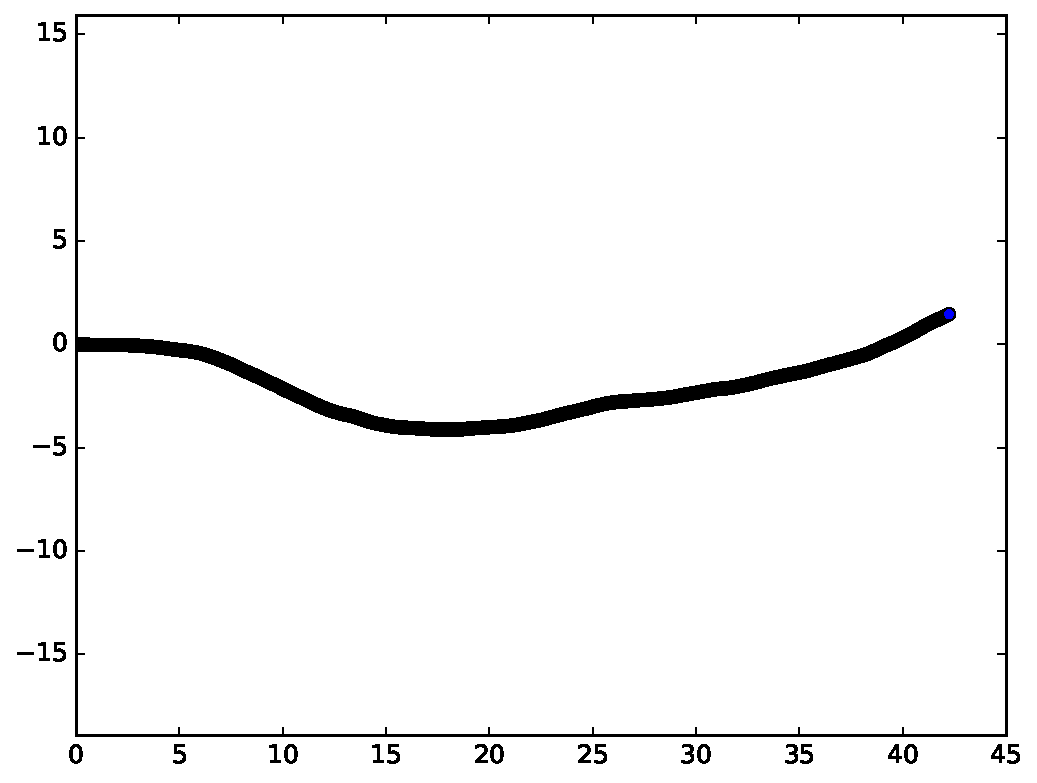
\includegraphics[width=\textwidth]{figures/ch4/ac_2_19_1_120a}
			\caption[Mouvement pseudo-autocorrélé A]{$F = 120$ et $A = 1$.}
			\label{fig:ac1_120A}
		\end{subfigure}
		~
		\begin{subfigure}[t]{0.49\textwidth}
			\centering
			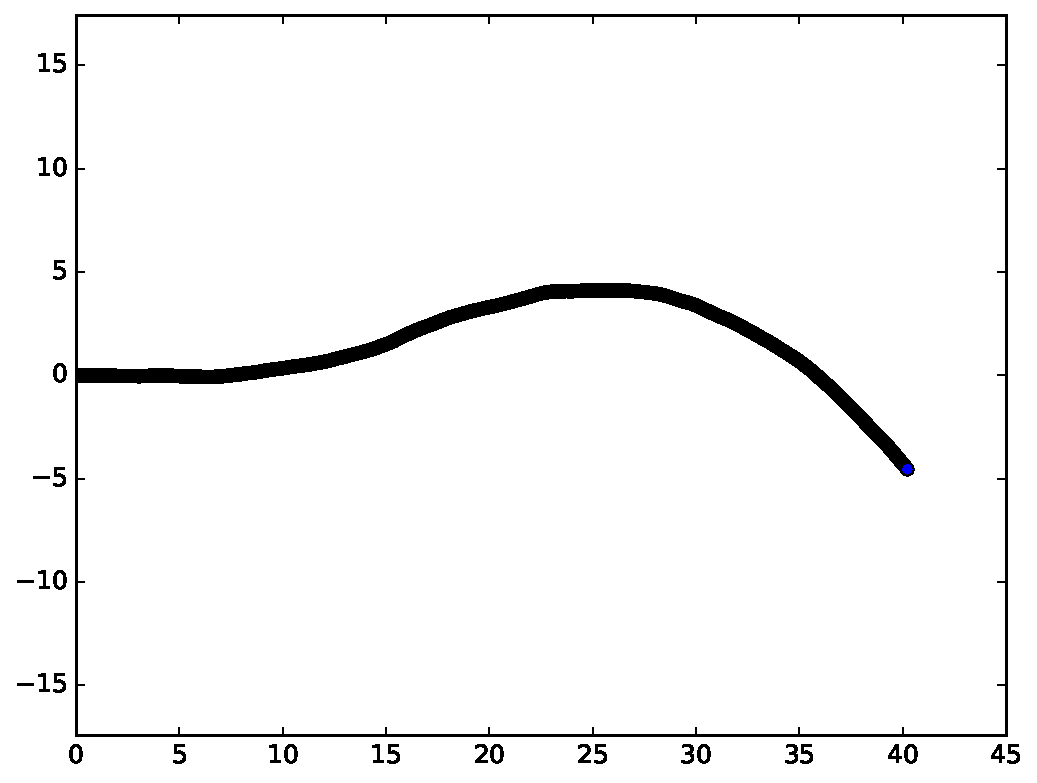
\includegraphics[width=\textwidth]{figures/ch4/ac_2_19_1_120b}
			\caption[Mouvement pseudo-autocorrélé B]{$F = 120$ et $A = 1$, bis.}
			\label{fig:ac_1_120B}
		\end{subfigure}
		~
		\begin{subfigure}[t]{0.49\textwidth}
			\centering
			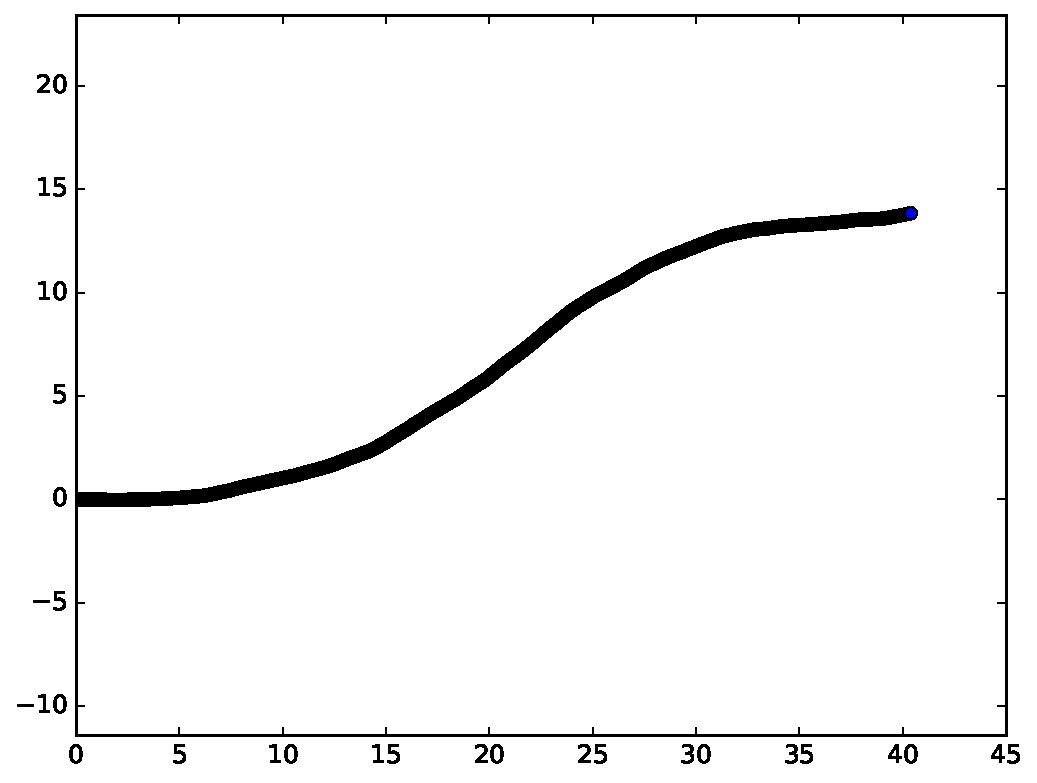
\includegraphics[width=\textwidth]{figures/ch4/ac_2_19_2_30}
			\caption[Mouvement pseudo-autocorrélé B]{$F = 30$ et $A = 2$.}
			\label{fig:ac_2_30}
		\end{subfigure}		
		~
		\begin{subfigure}[t]{0.49\textwidth}
			\centering
			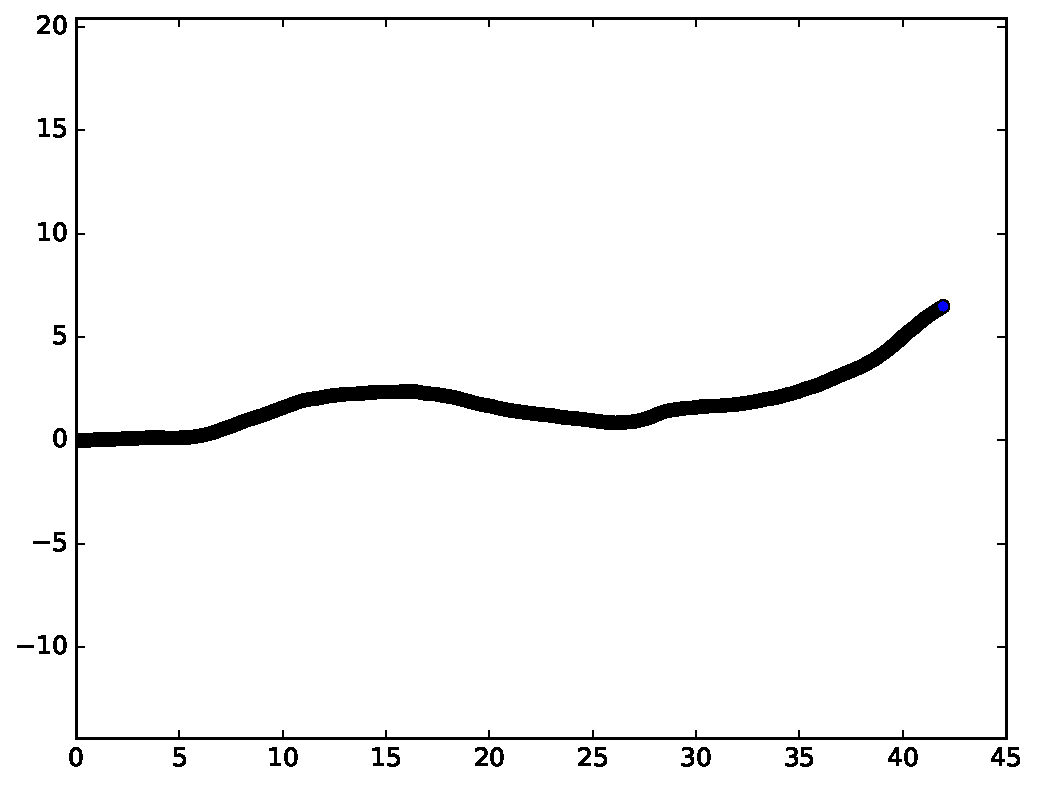
\includegraphics[width=\textwidth]{figures/ch4/ac_2_19_2_60}
			\caption[Mouvement pseudo-autocorrélé B]{$F = 120$ et $A = 1$, ter.}
			\label{fig:ac_1_120C}
		\end{subfigure}
		\caption[Mouvements pseudo-autocorrélés]{Trois trajectoires générées avec les mêmes valeurs $F = 120$~Hz et $A = 1\degree$, et une avec $F = 30$~Hz et $A = 2\degree$. Dans tous les cas, $V = 2,19$~cm/s. Ces trajectoires ressemblent à celles que l'on pourrait attendre d'objets autocorrélés, tels que des véhicules, par exemple.}
		\label{fig:autocorr}
	\end{figure}
    
    \subsection{Proposition de modèles de génération de mouvements autocorrélés}
    Les objets autocorrélés présentent néanmoins un intérêt certain, et les trajectoires pseudo-autocorrélées ne sont que des approximations qui peuvent s'avérer unsuffisantes. Ces objets pourraient faire l'objet d'études spécifiques pour lequelles de telles approximations ne seraient pas suffisantes. Nous proposons donc ici deux modèles différents permettant de générer des mouvements réellement autocorrélés.
    
    \subsubsection{Modèle VFA à mémoire}
    Une première option pour un modèle adapté aux objets autocorrélés serait d'adapter le modèle VFA en lui ajoutant une mémoire, par exemple une mémoire du dernier changement de direction de l'objet concerné. L'on retiendrait ainsi l'angle du changement de direction à l'instant précédent ($\alpha_{t-T}$, avec $T = \frac{1}{F}$), et l'on pourrait appliquer un nouveau changement avec un angle plus ou moins proche de ce dernier, selon des paramètres. L'équation~\ref{eq:vfamem} présente une possibilité, où $\alpha$ est échantilloné entre $-A$ et $+A$, et $c_{ac} \in [0,1]$ est un coefficient d'autocorrélation.
    
    \begin{equation}
		\alpha_{t} = \alpha_{t-T} \times c_{ac} + \alpha (1 - c_{ac})
		\label{eq:vfamem}
    \end{equation}
    
	Ainsi, lorsque le coefficient d'autocorrélation est nul, le système devient markovien ; lorsqu'il vaut 1, $\alpha_{nT}$ est constant (avec $n \in \mathbb{N}$). De fait, s'il est non nul, l'objet aura un mouvement circulaire s'il est ciné-continu et régulier s'il est ciné-discret , s'il est nul, le mouvement sera rectiligne dans les deux cas.
    
    \subsubsection{Modèle newtonien}
    Une seconde option ayant le mérite d'avoir un certain sens physique consisterait à considérer chaque objet comme une particule dotée d'une masse, et de la soumettre à une force qui, elle, serait régie par un modèle de type VFA, éventuellement modifié pour remplacer la vitesse par la norme de la force, notamment. Sans doute serait-il également opportun d'appliquer une force de friction afin d'éviter que l'application (même approximativement) constante d'une force (et donc d'une accélération\footnotemark{}) ne mène à des vitesses potentiellement croissantes et non bornées.
    
    \footnotetext{Rappelons que, d'après la seconde loi de Newton~\cite{newton1833philosophiae}, $\vec{F} = m\vec{a}$ où $F$ est une force, $m$ est la masse de l'objet sur lequel elle agit, et $\vec{a}$ est l'accélération de l'objet, soit $\vec{a} = \frac{\vec{F}}{m}$, où l'on voit bien que l'application d'une force constante à un objet de masse constante mène à une accélération constante, donc à une vitesse croissant linéairement. En l'absence de résistance à $\vec{F}$, la vitesse n'est pas bornée.}
    
    Le modèle nécessiterait un calibrage précis pour obtenir le comportement souhaité, notamment en ce qui concerne les masses des objets ou le coefficient de friction. Notons par ailleurs que, sauf dans certains cas particuliers (et après une période dynamique) les vitesses des objets ne seraient pas constantes pour une norme de $\vec{F}$ donnée, ce qui distinguerait ce modèle newtonien du nôtre (VFA). En soi, ce n'est pas nécessairement un problème --- et peut même être un avantage --- mais cela complique le contrôle des propriétés d'un environnement synthétique créé pour mener une étude empirique.

\section{Expérience et protocole}
	Nous avons mené une étude empirique visant à évaluer les performances de sélection de cibles mobiles en fonction de la nature du mouvement. Nous avions 13 sujets, âgés de 14 à 56 ans. Ils avaient pour tâche de cliquer sur une cible mobile (un disque) affichée sur un écran d'ordinateur de bureau.

	\subsection{Dispositif expérimental}
	Le périphérique de saisie était une souris standard sans accélération, afin d'éviter le biais potentiel introduit par une fonction de gain pouvant être familière pour certains utilisateurs et pas pour d'autres. Cette souris pilotait un curseur cruciforme gris. Le moniteur était un Dell \emph{UltraSharp U2412M}\footnotemark{}, de 24 pouces (60,96~cm) de diagonale, et d'environ 94 pixels par pouce (37 pixels par cm).
	
	La tâche elle-même était toutefois limitée à une fenêtre carrée de 1000 pixels de côté, soit 26,92~cm.

	\footnotetext{\url{http://www.dell.com/en-us/work/shop/cty/pdp/spd/dell-u2412m}}

	\subsection{Tâche et conditions}
	\subsubsection{Description de la tâche}
	La tâche consistait à sélectionner une cible parmi 50 objets identiques : des disques de 5,4~mm de diamètre. Les 49 \og distracteurs \fg{} étaient affichés en gris, et la cible à sélectionner était rouge, comme l'illustre la figure~\ref{fig:app}. Les distracteurs et la cible étaient mus selon les mêmes paramètres V, F et A de notre modèle, mais l'angle $\alpha$ échantillonné à chaque période T était échantillonné séparément pour chaque objet, donc généralement différent. Lorsqu'un disque \og percutait \fg{} le bord de la fenêtre, il \og rebondissait \fg{} dessus.
	
	\begin{figure}[!htb]
		\centering
		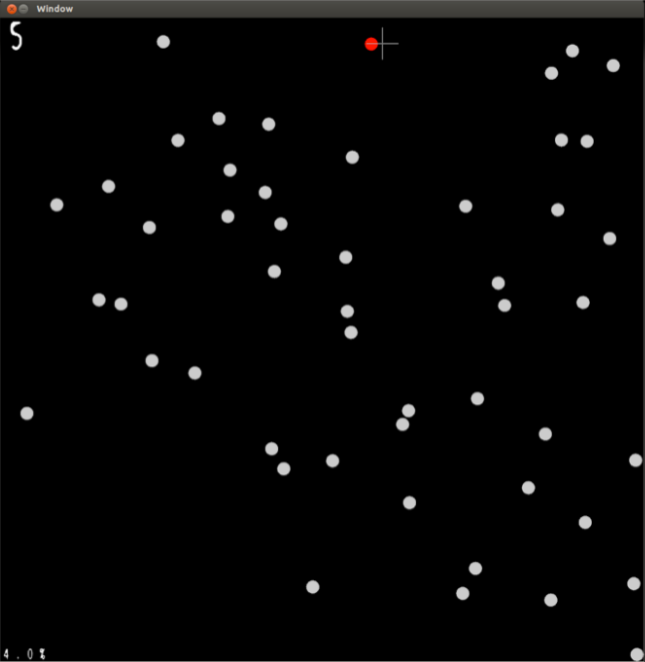
\includegraphics[width=\textwidth]{figures/ch4/app}
		\caption[Application utilisée dans notre évaluation]{Application utilisée dans notre évaluation. Le curseur gris s'approche de la cible rouge (qui n'est pas sélectionnable ici, car le centre du curseur cruciforme n'est pas inclus dans le disque) et les distracteurs gris se déplacent dans la fenêtre. Le nombre de tentatives de sélection encore possibles pour la cible courante est affiché en haut à gauche --- 5 dans le cas présent. Le taux de complétion de l'expérience dans son ensemble est inscrit en bas à gauche.}
		\label{fig:app}
	\end{figure}
	
	Ce choix, qui altère ponctuellement le mouvement généré par le modèle VFA, fut fait pour d'une part éviter la disparition d'une cible hors de la fenêtre, pour éviter toute discontinuité (par exemple si la cible réapparaissait de l'autre côté de la fenêtre), et pour limiter la \og surprise \fg{} éprouvée par l'utilisateur en imitant un phénomène physique familier. Cela permet par ailleurs de garantir la constance la densité de l'environnement.
	
	Pour contrôler l'amplitude (telle que définie par Fitts~\cite{fitts1954information}) les mouvements des distracteurs étaient légèrement contraints, de telle sorte qu'après la sélection d'une cible, la distance entre le curseur et la cible suivante était à peu près constante (environ 7,96~cm).
	
	Quand une cible était sélectionnée avec succès, elle changeait brièvement de couleur pour devenir verte tandis que la cible suivante devenait rouge.
	
	\subsubsection{Erreurs et échecs}
	La sélection de cibles implique un compromis entre vitesse et précision~\cite{guiard2011fitt}, et les utilisateurs sont généralement libres d'adopter différentes approches de ce compromis, privilégiant le premier ou le second objectif. Il peut en résulter, d'un utilisateur à l'autre, d'importants écarts de temps de sélection et de taux d'erreurs. Afin de minimiser ces variations, nos sujets avaient pour instruction de sélectionner leurs cibles le plus rapidement possible, mais avec un maximum de 5 tentatives.
	
	Le nombre de tentatives encore possible était affiché dans le coin supérieur gauche de la fenêtre (voir la figure~\ref{fig:app}). Après la dernière tentative, en cas d'échec le mot \emph{failure} était affiché à la place du nombre de tentatives, indiquant un échec. Mais les sujets avaient pour instruction de continuer à essayer de sélectionner la cible, sans plus chercher à minimiser les erreurs. Cette particularité de notre dispositif expérimental était nécessaire pour avoir suffisamment de données (en temps de sélection) pour les conditions les plus difficiles, qui généraient énormément d'erreurs.
	
	Elle a néanmoins l'inconvénient de réduire quelque peu les temps de sélection des conditions les plus difficiles, tout en augmentant leurs taux d'erreurs. Ainsi, les échecs ne sont pas absolus, mais indiquent les conditions pour lesquelles la sélection est (parfois extrêmement) difficile.
	
	\subsubsection{Conditions évaluées}
	Nous avons testé toutes les combinaisons des valeurs de V, F et A suivantes, avec 4 sélections par condition et par sujet :
	
	\begin{description}
		\item[V :] 0,73, 1,46 et 2,19~cm/s, soit 3 valeurs ;
		\item[F :] 1, 2, 4, 8, 13, 20 et 30~Hz, soit 7 valeurs ;
		\item[A :] 0, 30, 60, 90, 120 et 180 degrés, soit 6 valeurs.
	\end{description}
	
	À ceci s'ajoutait une condition de base avec des cibles statiques, répétée 20 fois. Naturellement, lorsque $A = 0$, les cibles se déplacent en ligne droite. Au total, nous avons évalué $3 \times 7 \times 6 + 1 = 127$ conditions ave 4 essais par condition dynamique et 20 essais pour la condition statique, soit un total de $126 \times 4 + 1 \times 120 = 524$ essais par participant, et $524 \times 13 = 6812$ essais au total.
	
	La conception de ce protocole impliquait un compromis difficile entre plusieurs objectifs contradictoires : avoir suffisamment de conditions pour évaluer un échantillon représentatif des types de mouvements possibles, avoir suffisamment de données par condition pour avoir des résultats fiables, limiter l'évaluation dans le temps et dans l'intensité pour limiter la fatigue des sujets et ne pas les décourager.
	
	\paragraph{Choix des valeurs évaluées.}
	Les valeurs de V (dont la deuxième est le double de la première, et la troisième le triple) furent choisies pour avoir une vitesse faible générant des sélections faciles, une vitesse intermédiaire, et une vitesse élevée générant des conditions difficiles.
	
	Les valeurs de F furent choisies pour couvrir l'espace des fréquences qu'un utilisateur peut percevoir comme significativement différentes. Nous avons en effet observé au cours de plusieurs études pilotes que l'augmentation de la fréquence au-delà de 30~Hz n'était pas très sensible, mais que de petites différences absolues pouvaient être significatives si elles étaient relativement grandes ; par exemple, passer de 1~Hz à 2~Hz revient à n'ajouter qu'un seul hertz, mais à doubler la fréquence. Il était donc nécessaire d'avoir une plus forte densité de valeurs testées dans les basses fréquences que dans les hautes.
	
	Les valeurs de A résultent d'un constat similaire, mais moins marqué. Ainsi, les valeurs évaluées vont simplement de 0\textdegree{} à 180\textdegree{} par pas de 30\textdegree{} ; la valeur 150\textdegree{} est omise car trop similaire (subjectivement) aux valeurs 120\textdegree{} et 180\textdegree{}, et afin de limiter le nombre de conditions.

	\subsection{Procédure et collecte de données}
	\subsubsection{Descrption de la procédure}
	Chaque session durait environ 40 minutes (selon les performances du sujet) dont une phase d'entraînement de plus de 50 essais, prenant fin au moment où le sujet se sentait suffisamment à l'aise pour commencer l'évaluation.
	
	Des pauses d'une durée laissée au choix du sujet étaient accordées à 25~\%{}, 50~\%{} et 75~\%{} de complétion de l'évaluation, afin de limiter les effets de la fatigue. Permettons-nous en effet d'insister sur le fait que la tâche nécessite une concentration intense et soutenue, en plus d'un effort physique non négligeable compte tenu de la rapidité et de la précision requises. Les pauses étaient donc généralement appréciées.
	
	À la fin de l'évaluation, un court questionnaire était soumis aux sujets afin de recueillir leurs impressions subjectives sur les différentes \og classes \fg{} de mouvements qu'ils étaient capables d'identifier, et les éventuelles stratégies qu'ils avaient pu mettre en place pour chaque classe.
	
	\subsubsection{Données collectées}
	Pour chaque essai, nous avons mesuré :
	
	\begin{description}
		\item[Le temps de sélection :] entre l'instant où la cible devient rouge et celui où elle est effectivement sélectionnée,
		\item[Les erreurs :] le nombre de clics hors de la cible,
		\item[Les échecs :] lorsqu'une tâche engendre au moins cinq erreurs,
		\item[La position de la cible] tout au long de la tâche,
		\item[La position du curseur,] également tout au long de la tâche.
	\end{description}

\section{Résultats : performances de sélection}
	Les valeurs présentées ici sont des moyennes calculées sur l'ensemble de nos sujets.
	
	\subsection{Temps de sélection}
	Les performances de sélection dans les conditions les plus faciles étaient relativement stable d'un sujet à l'autre : le plus lent fut moins de quatre fois plus lent que le plus rapide pour le mouvement rectiligne. Cependant, pour les conditions les plus difficiles, les écarts peuvent être considérables, d'un facteur supérieur à 18 du sujet le plus rapide au plus lent.
	
	\subsubsection{Temps de sélection normalisés}
	Par conséquent, et pour éviter d'accorder trop de poids aux sujets les plus lents, nous avons choisi de normaliser les temps de sélection par sujet. Ainsi, pour chaque sujet, le temps de sélection normalisé (TSN) est la moyenne des temps de sélection par condition, normalisée selon la condition la plus difficile \emph{pour le sujet en question}.
	
	Par exemple, si une condition a un TSN de 0,75 pour un sujet donné, cela signifie qu'il a fallu à ce sujet (en moyenne sur les 4 essais) 75~\%{} du temps dont il a eu besoin (en moyenne sur les 4 essais) pour la condition qui lui a demandé le plus de temps. La moyenne des temps de sélection normalisés (MTSN) d'une condition est donc la moyenne des TSN de tous les sujets pour cette condition.
	
	Attendu que la condition la plus difficile n'est pas nécessairement la même pour tous les sujets, aucune condition n'a une MTSN de 1,0.
	
	\subsection{Erreurs et échecs}
	\subsubsection{Erreurs}
	Le nombre d'erreurs est compris entre 0 et 5 (les clics erronés ne sont pas comptabilisés après le cinquième, attendu que les sujets ont dans ce cas pour instruction de ne pas chercher à éviter les erreurs --- ils sont toutefois enregistrés). Un taux d'erreur (TERR) de 3,5 pour une condition donnée signifie donc qu'en moyenne, les sujets ont fait 3,5 clics hors de la cible pour ladite condition.
	
	\subsubsection{Échecs}
	Un échec survient lorsque pour une tâche de sélection, un sujet commet au moins 5 erreurs. 	Un taux d'échecs (TECH) de 50~\%{} pour une condition donnée signifie que la moitié des essais pour cette condition ont mené à un échec (5 clics erronés ou plus) sur l'ensemble des sujets.
	
	Notez que du fait d'inquiétudes croissantes dans divers domaines de recherche concernant les limites des tests de significativité d'hypothèse nulle~\cite{dragicevic2014running, cumming2014new}, nos analyses se fondent principalement sur les tailles d'effets, rapportés ici sous forme de différences de pourcentage $p$, calculées selon la formule suivante, pour deux mesures $m_{1}$ et $m_{2}$ : $p = 100 \times \frac{\abs*{m_{2} - m_{1}}}{\frac{m_{1} + m_{2}}{2}}$.

	\subsection{Vitesse}
	Sans surprise, les temps de sélection et les taux d'erreurs croissent avec la vitesse des cibles, comme l'illustre la figure~\ref{fig:spEffectPerf}. Ainsi, la moyenne des MTSN de toutes les conditions lentes (0,73~cm/s) est de 16,74~\%{}, celle des conditions de vitesse intermédiaire est de 25,02~\%{}, et celle des conditions rapides est de 36,58~\%{}. Les différences de pourcentages croisées entre ces conditions sont présentées dans le tableau~\ref{tab:spPerf}.

	Les MTSN, TERR et TECH en fonction de la vitesse sont présentés sur la figure~\ref{fig:spEffectPerf}, pour des valeurs de A de 60 et 120, et pour toutes les valeurs de F. Les conditions associées aux autres valeurs de A sont omises ici, dans un souci de concision, mais présentent des caractéristiques très similaires.
	
%	\newcommand{\newrow}{\bigstrut[t] \\ \hline}
	\begin{table}
		\centering
		\begin{tabular}{r c | c c c}
			Vitesse			&			& Basse		& Moyenne	& Haute		\bigstrut[b] \\
							&			& (16,74)	& (25,02)	& (36,58)	\bigstrut[b] \\ \hline
			Basse			& (16,74)	& 0,00		& 39,65		& 74,40		\bigstrut[t] \\
			Moyenne			& (25,02)	& 39,65		& 0,00		& 37,51		\\
			Haute			& (36,58)	& 74,40		& 37,51		& 0,00		\\
		\end{tabular}
		\caption[Performances selon la vitesse]{Performances de sélection (MTSN moyennes) selon la vitesse, et différences de pourcentages. Les MTSN moyennes associées à chaque vitesse sont présentées sur la première ligne et la première colonne en pourcentages, et les différences de pourcentages croisées sont indiquées à l'intérieur du tableau.}
		\label{tab:spPerf}
	\end{table}
	
	On observe que les MTSN et TERR sont approximativement des fonctions affine de la vitesse, pour une pseudo-entropie (i.e., le produit AF) donnée. Les TECH tendent à croître de façon super-linéaire, probablement du fait de l'effet de seuil introduit par notre définition (arbitraire) d'un échec.

	\newcommand{\subImgWlineplot}{0.48\textwidth}
	\begin{figure}[!htb]
		\centering
		\begin{subfigure}[t]{\subImgWlineplot}
			\centering
			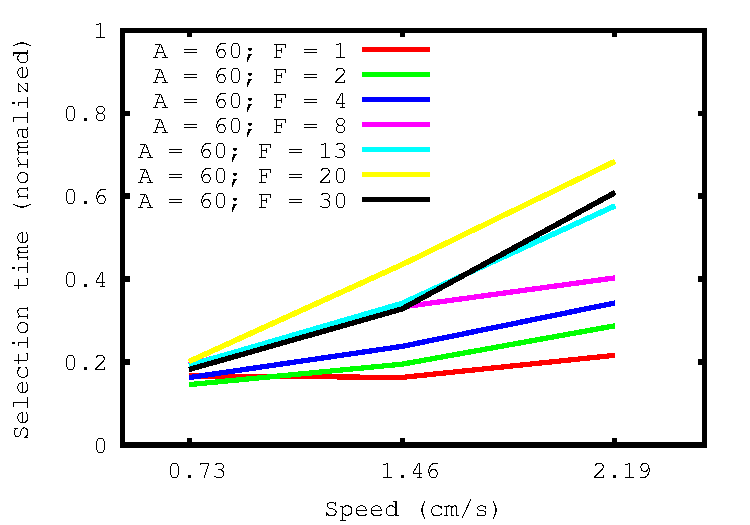
\includegraphics[width=\textwidth]{figures/ch4/speed_angle_60_times}
			\caption{MTSN pour $A = 60$.}
			\label{fig:spEffect_t_60}
		\end{subfigure}
		~
		\begin{subfigure}[t]{\subImgWlineplot}
			\centering
			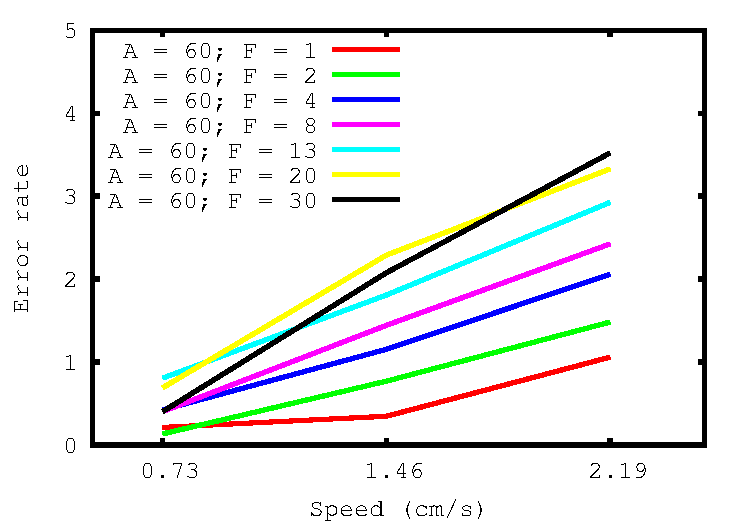
\includegraphics[width=\textwidth]{figures/ch4/speed_angle_60_errors}
			\caption{Taux d'erreurs pour $A = 60$.}
			\label{fig:spEffect_e_60}
		\end{subfigure}
		~
		\begin{subfigure}[t]{\subImgWlineplot}
			\centering
			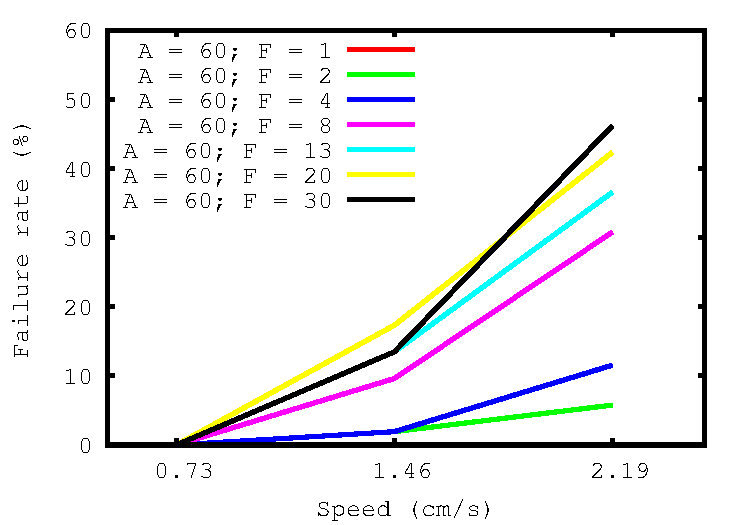
\includegraphics[width=\textwidth]{figures/ch4/speed_angle_60_failures}
			\caption{Taux d'échecs pour $A = 60$.}
			\label{fig:spEffect_f_60}
		\end{subfigure}
		~
		\begin{subfigure}[t]{\subImgWlineplot}
			\centering
			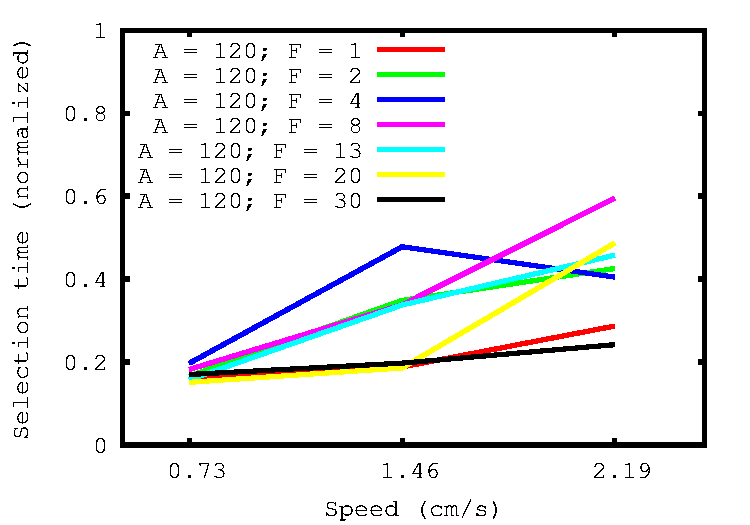
\includegraphics[width=\textwidth]{figures/ch4/speed_angle_120_times}
			\caption{MTSN pour $A = 120$.}
			\label{fig:spEffect_t_120}
		\end{subfigure}
		~
		\begin{subfigure}[t]{\subImgWlineplot}
			\centering
			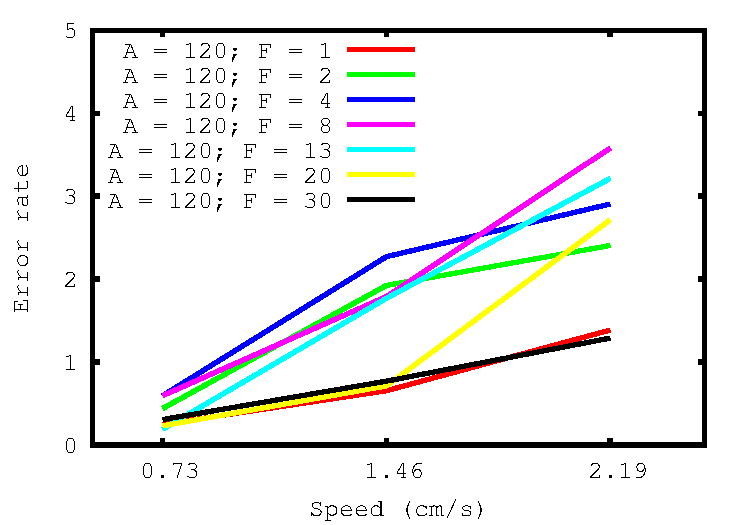
\includegraphics[width=\textwidth]{figures/ch4/speed_angle_120_errors}
			\caption{Taux d'erreurs pour $A = 120$.}
			\label{fig:spEffect_e_120}
		\end{subfigure}
		~
		\begin{subfigure}[t]{\subImgWlineplot}
			\centering
			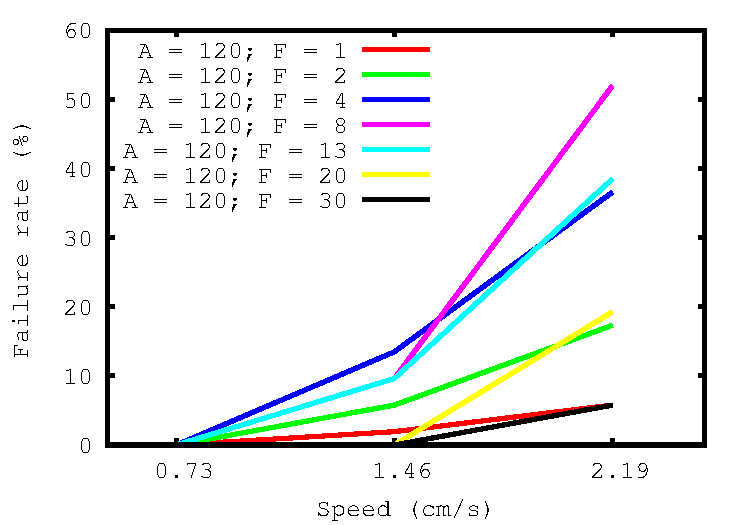
\includegraphics[width=\textwidth]{figures/ch4/speed_angle_120_failures}
			\caption{Taux d'échecs pour $A = 120$.}
			\label{fig:spEffect_f_120}
		\end{subfigure}
		\caption[Effet de la vitesse sur les performances de sélection]{Effet de la vitesse sur les performances de sélection. Les MTSN, taux d'erreurs d'échecs sont présentés pour deux valeurs de A, et pour toutes les valeurs de F que nous avons testées.}
		\label{fig:spEffectPerf}
	\end{figure}


	\subsection{Angle}
	L'effet du paramètre d'angle est plus subtile à interpréter, notamment du fait d'intéractions avec la vitesse et la fréquence. À basse vitesse, l'effet de A sur les MTSN est faible : pour $V = 0,73$ et $F = 4$, quand $A= 0$, $MTSN = 14~\%{}$ alors que quand $A = 120$, $MTSN = 20~\%{}$, soit une différence de pourcentage de seulement 33~\%{}, et qui plus est la plus importante mesurée entre deux valeurs de A pour cette vitesse. En revanche, lorsque S vaut 2,19, alors les MTSN sont respectivement 21~\%{} et 54~\%{} pour les mêmes valeurs de A et F, ce qui représente une différence de pourcentage de 90~\%{}.
	
	L'inteprétation que nous proposons est qu'à basse vitesse, la sélection est de toute façon relativement facile, presque indépendamment de la nature du mouvement, ce qui n'est plus du tout vrai avec des cibles rapides. Ces résultats sont illstrés par la figure~\ref{fig:aEffectPerf}.

	\begin{figure}[!htb]
		\centering
		\begin{subfigure}[t]{\subImgWlineplot}
			\centering
			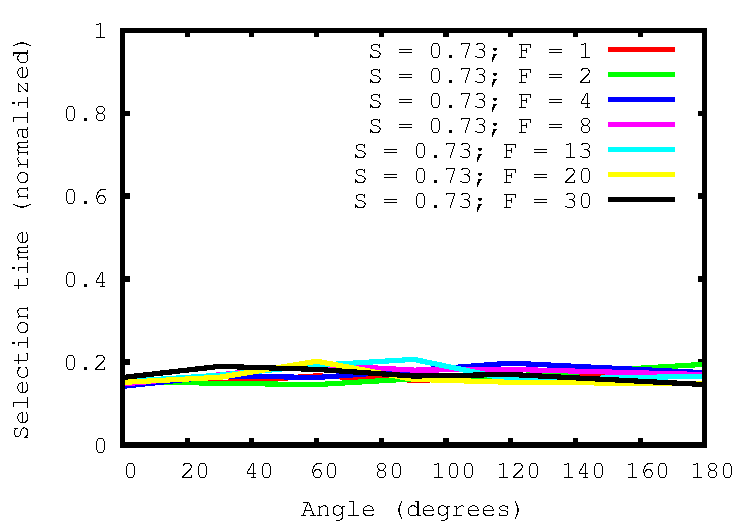
\includegraphics[width=\textwidth]{figures/ch4/angle_speed_0_73_times}
			\caption{MTSN pour $V = 0,73$.}
			\label{fig:aEffect_t_073}
		\end{subfigure}
		~
		\begin{subfigure}[t]{\subImgWlineplot}
			\centering
			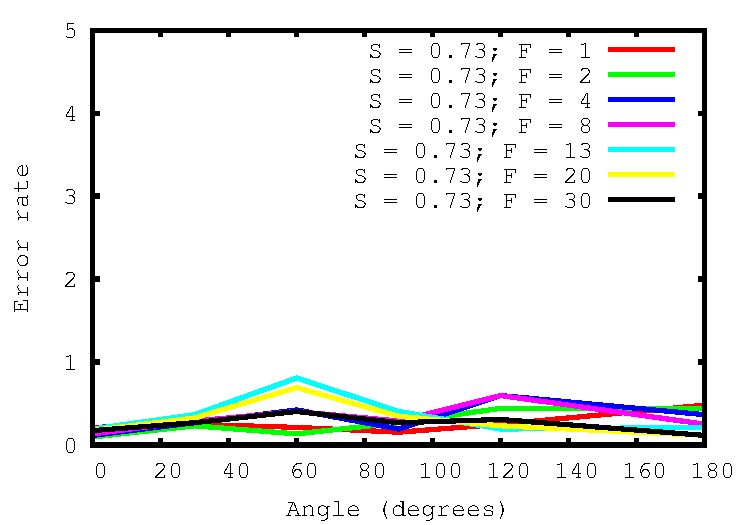
\includegraphics[width=\textwidth]{figures/ch4/angle_speed_0_73_errors}
			\caption{Taux d'erreurs pour $V = 0,73$.}
			\label{fig:aEffect_e_073}
		\end{subfigure}
		~
		\begin{subfigure}[t]{\subImgWlineplot}
			\centering
			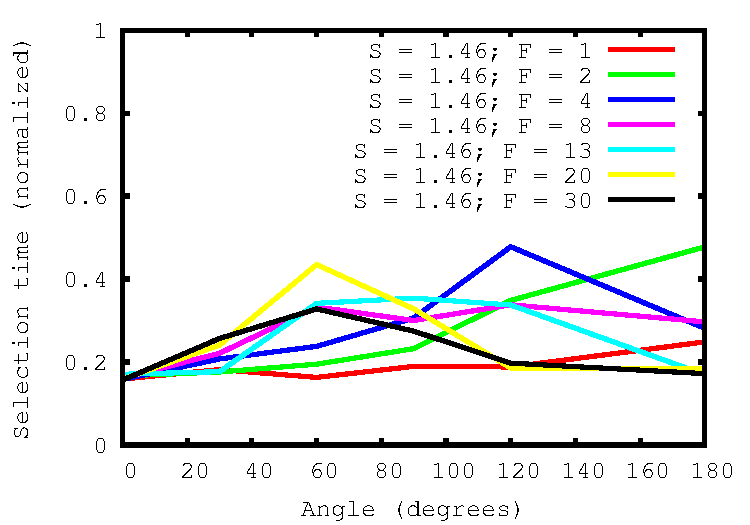
\includegraphics[width=\textwidth]{figures/ch4/angle_speed_1_46_times}
			\caption{MTSN pour $V = 1,46$.}
			\label{fig:aEffect_t_146}
		\end{subfigure}
		~
		\begin{subfigure}[t]{\subImgWlineplot}
			\centering
			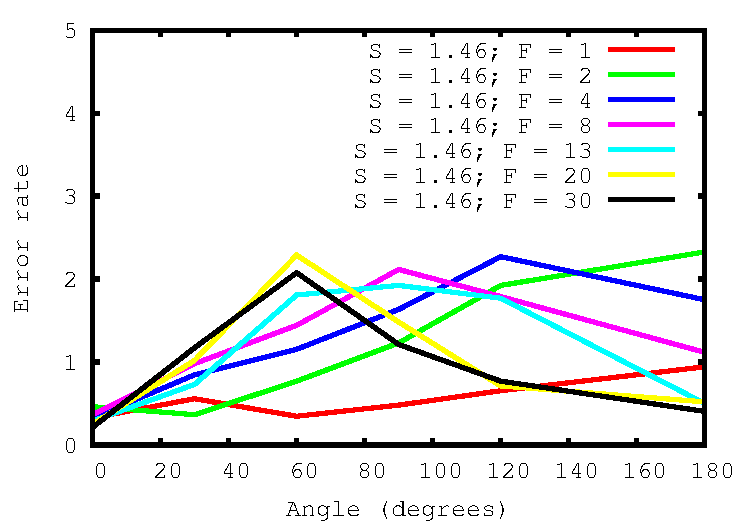
\includegraphics[width=\textwidth]{figures/ch4/angle_speed_1_46_errors}
			\caption{Taux d'erreurs pour $V = 1,46$.}
			\label{fig:aEffect_e_146}
		\end{subfigure}
		~
		\begin{subfigure}[t]{\subImgWlineplot}
			\centering
			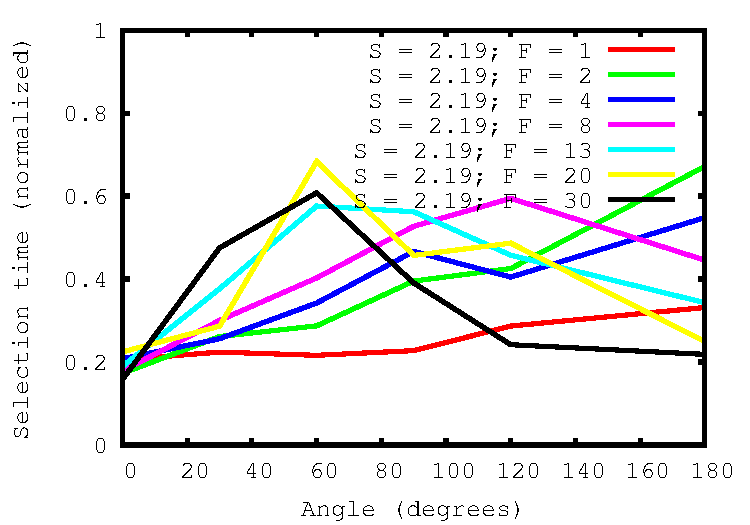
\includegraphics[width=\textwidth]{figures/ch4/angle_speed_2_19_times}
			\caption{MTSN pour $V = 2,19$.}
			\label{fig:aEffect_t_219}
		\end{subfigure}
		~
		\begin{subfigure}[t]{\subImgWlineplot}
			\centering
			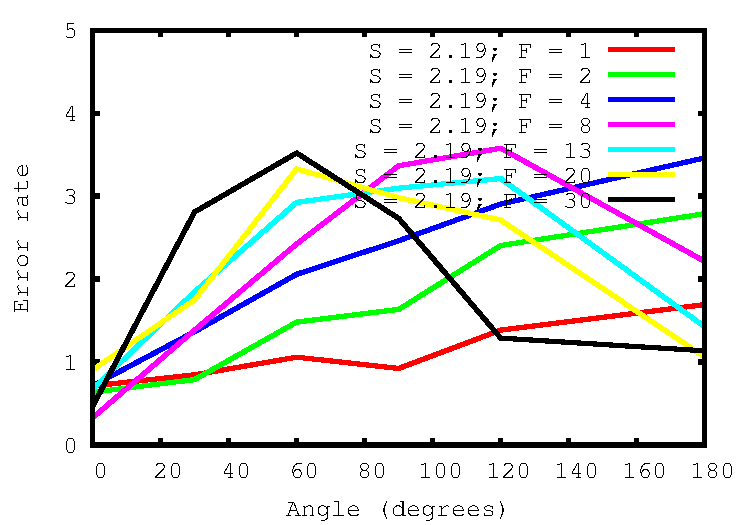
\includegraphics[width=\textwidth]{figures/ch4/angle_speed_2_19_errors}
			\caption{Taux d'erreurs pour $V = 2,19$.}
			\label{fig:aEffect_e_219}
		\end{subfigure}
		\caption[Effet du paramètre d'angle sur les performances de sélection]{Effet du paramètre d'angle sur les performances de sélection. Les MTSN et taux d'erreurs sont présentés pour toutes les valeurs de V et de F que nous avons testées. Comme on le voit, les interactions sont fortes entre les différents paramètres, et les effets de A et F sont d'autant plus marqués que V est grande.}
		\label{fig:aEffectPerf}
	\end{figure}
	
	En particulier, la figure~\ref{fig:aEffect_t_219} montre l'effet de A sur les MTSN à haute vitesse. Observons que tant que la fréquence est basse, de faibles valeurs de A sont associées à de faibles MTSN ; mais lorsque F croît, l'effet de A sur les temps de sélection change : les MTSN croissent d'abord avec A, atteignent un plateau, puis décroissent.
	
	De plus, la valeur de A associée à ce plateau ($A_{pic}$) dépend de A : plus F est grande, plus $A_{pic}$ est petit. Les erreurs et les échecs (omis ici) suivent la même tendance, mais les effets sont dépendants de la vitesse (d'autant plus forts qu'elle est élevée).

	\subsection{Fréquence}
	Les tendances sont similaires pour la fréquence : F a un plus petit impact sur le temps de sélection lorsque la vitesse est basse, et plus grand quand elle est élevée. Sur la figure~\ref{fig:fEffectPerf}, on observe que lorsque A est faible, les fortes valeurs de F sont corrélées avec de longs temps de sélection. Mais pour de fortes valeurs de A, la tendance change : quand A est grand, la MTSN croît avec F jusqu'à une certaine valeur ($F_{pic}$), puis décroît. De plus, la valeur de $F_{pic}$ diminue quand A augmente. Les TERR et TECH suivent la même tendance que les MTSN.
	
	L'effet de F est donc approximativement symétrique de celui de A, et comme pour A, il est d'autant plus prononcé que la vitesse est élevée.

	\begin{figure}[!htb]
		\centering
		\begin{subfigure}[t]{\subImgWlineplot}
			\centering
			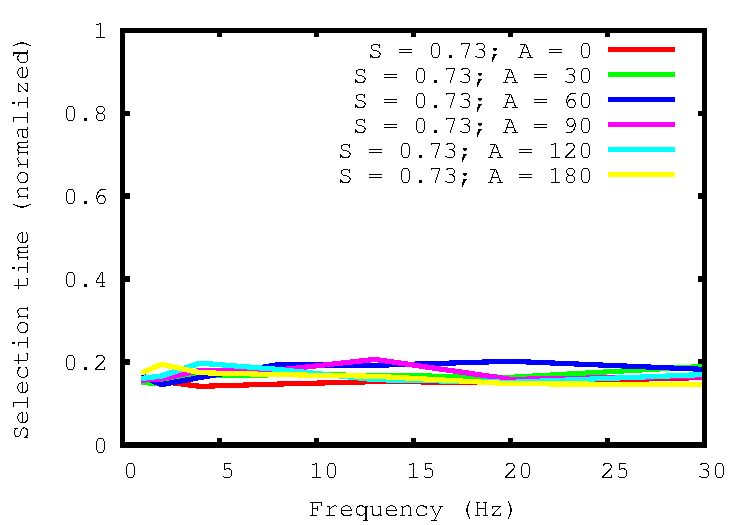
\includegraphics[width=\textwidth]{figures/ch4/frequency_speed_0_73_times}
			\caption{MTSN pour $V = 0,73$.}
			\label{fig:fEffect_t_073}
		\end{subfigure}
		~
		\begin{subfigure}[t]{\subImgWlineplot}
			\centering
			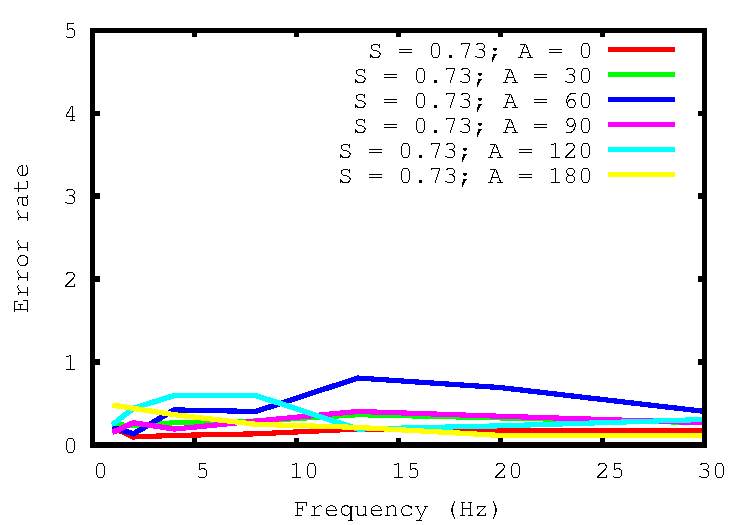
\includegraphics[width=\textwidth]{figures/ch4/frequency_speed_0_73_errors}
			\caption{Taux d'erreurs pour $V = 0,73$.}
			\label{fig:fEffect_e_073}
		\end{subfigure}
		~
		\begin{subfigure}[t]{\subImgWlineplot}
			\centering
			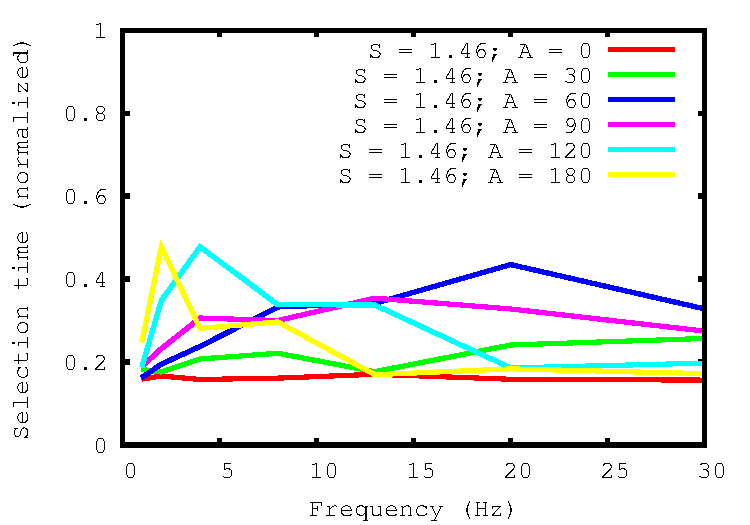
\includegraphics[width=\textwidth]{figures/ch4/frequency_speed_1_46_times}
			\caption{MTSN pour $V = 1,46$.}
			\label{fig:fEffect_t_146}
		\end{subfigure}
		~
		\begin{subfigure}[t]{\subImgWlineplot}
			\centering
			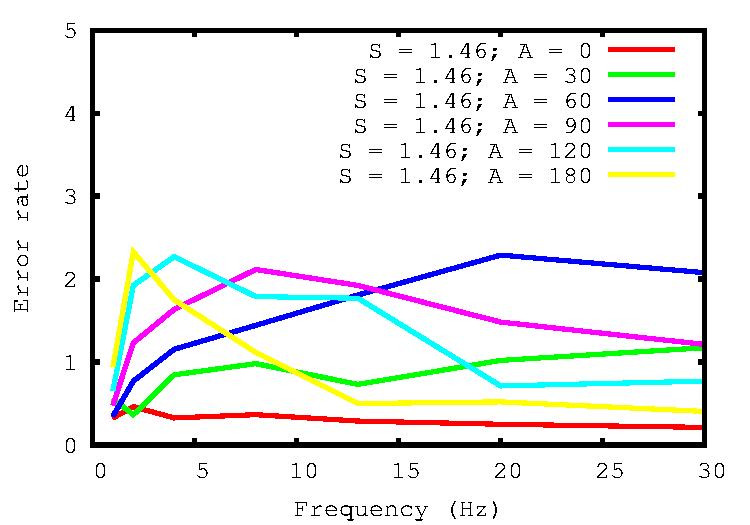
\includegraphics[width=\textwidth]{figures/ch4/frequency_speed_1_46_errors}
			\caption{Taux d'erreurs pour $V = 1,46$.}
			\label{fig:fEffect_e_146}
		\end{subfigure}
		~
		\begin{subfigure}[t]{\subImgWlineplot}
			\centering
			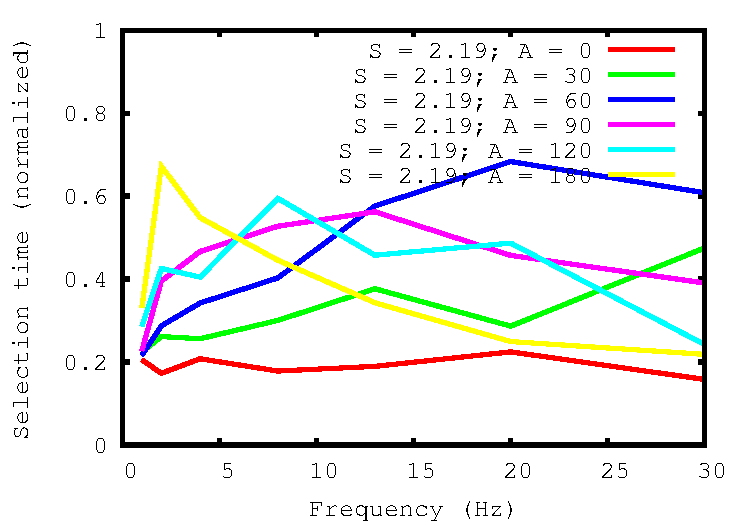
\includegraphics[width=\textwidth]{figures/ch4/frequency_speed_2_19_times}
			\caption{MTSN pour $V = 2,19$.}
			\label{fig:fEffect_t_219}
		\end{subfigure}
		~
		\begin{subfigure}[t]{\subImgWlineplot}
			\centering
			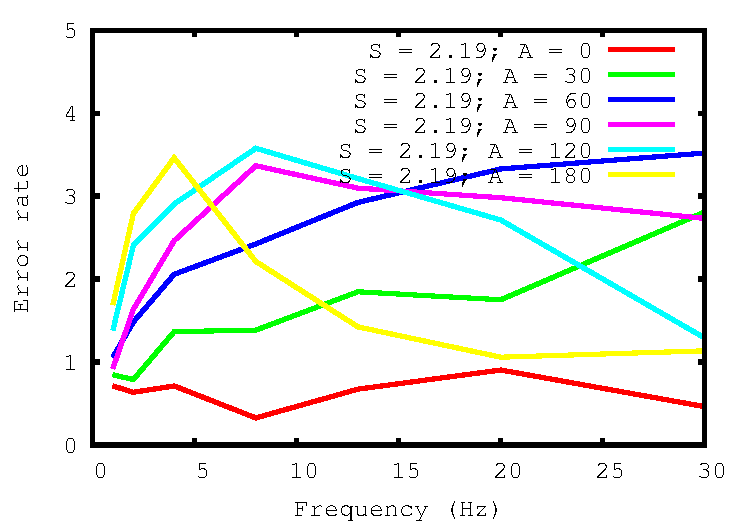
\includegraphics[width=\textwidth]{figures/ch4/frequency_speed_2_19_errors}
			\caption{Taux d'erreurs pour $V = 2,19$.}
			\label{fig:fEffect_e_219}
		\end{subfigure}
		\caption[Effet de la fréquence sur les performances de sélection]{Effet de la fréquence sur les performances de sélection. Les MTSN et taux d'erreurs sont présentés pour toutes les valeurs de V et de A que nous avons testées. Comme on le voit, les interactions sont fortes entre les différents paramètres, et les effets de A et F sont d'autant plus marqués que V est grande.}
		\label{fig:fEffectPerf}
	\end{figure}

\section{Analyse exploratoire}
	Nous avons également porté un regard sur notre espace de paramètres entier afin d'identifier des tendances plus générales.

	Les cartes thermiques (\emph{heat maps}) sur les figures~\ref{fig:hmap_t_146} et~\ref{fig:hmap_t_219} présentent les MTSN pour toutes les combinaisons de A et F aux vitesses intermédiaire et élevée, respectivement. Sur chaque carte, A se lit sur l'axe des abscisses, et F sur celui des ordonnées. Les TERR et TECH sont également représentés sur la figure~\ref{fig:hmaps}.
	
	Nous remarquons sur toutes ces cartes de chaleur --- et plus clairement à 2,19~cm/s --- qu'une zone approximativement située sur la diagonale principale (du coin supérieur gauche au coin inférieur droit) est associé aux MTSN, TERR et TECH les plus élevés, donc aux conditions les plus difficiles.
	
	Si l'on suit cette diagonale et que l'on se rapporte aux axes des abscisses et des ordonnées, l'on peut remarquer qu'elle est caractérisée soit par une forte valeur de A associée à une faible valeur de F, soit l'inverse, soit à des valeurs de A et F simultanément intermédiaires.
	
	Inversement, lorsque A et F sont simultanément faibles (coin inférieur gauche) ou simultanément élevés (coin supérieur droit) la sélection est relativement aisée.

	\begin{figure}[!htb]
		\centering
		\begin{subfigure}[t]{\subImgWlineplot}
			\centering
			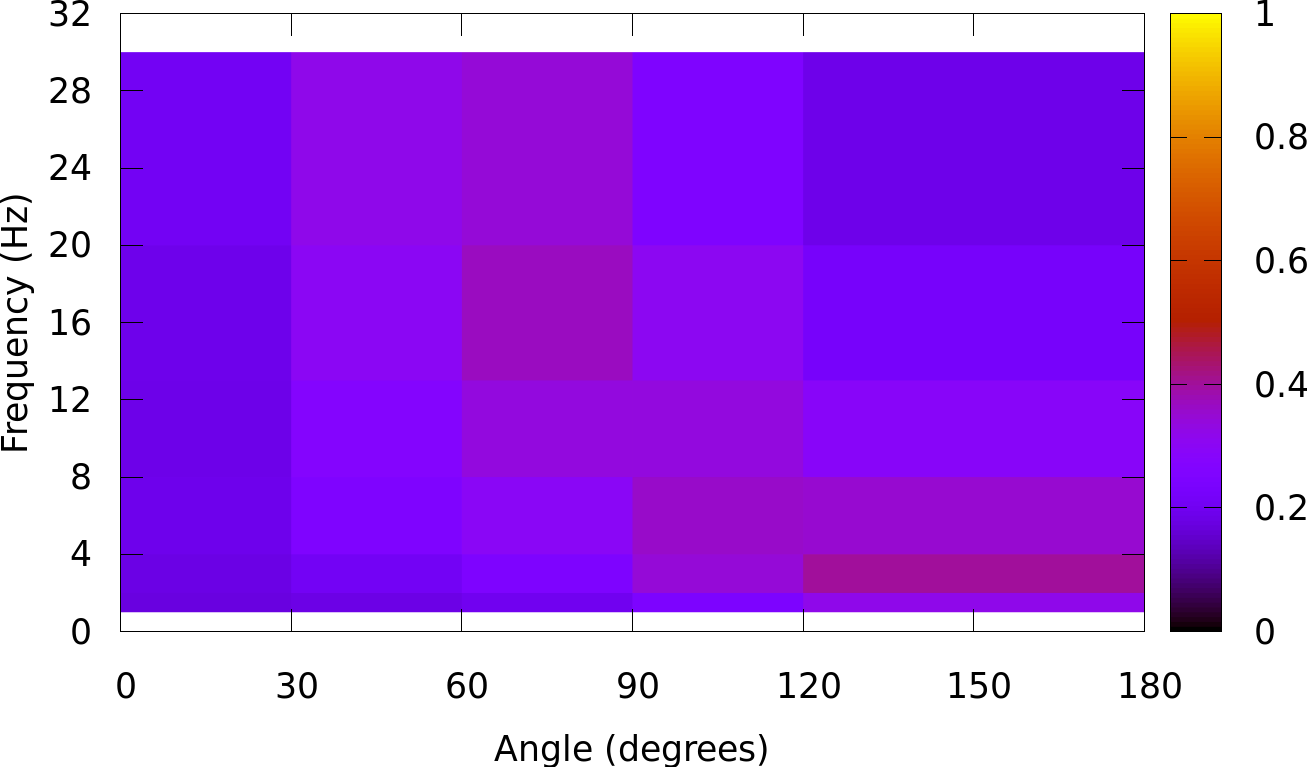
\includegraphics[width=\textwidth]{figures/ch4/average_times_054}
			\caption{MTSN pour $V = 1,46$.}
			\label{fig:hmap_t_146}
		\end{subfigure}
		~
		\begin{subfigure}[t]{\subImgWlineplot}
			\centering
			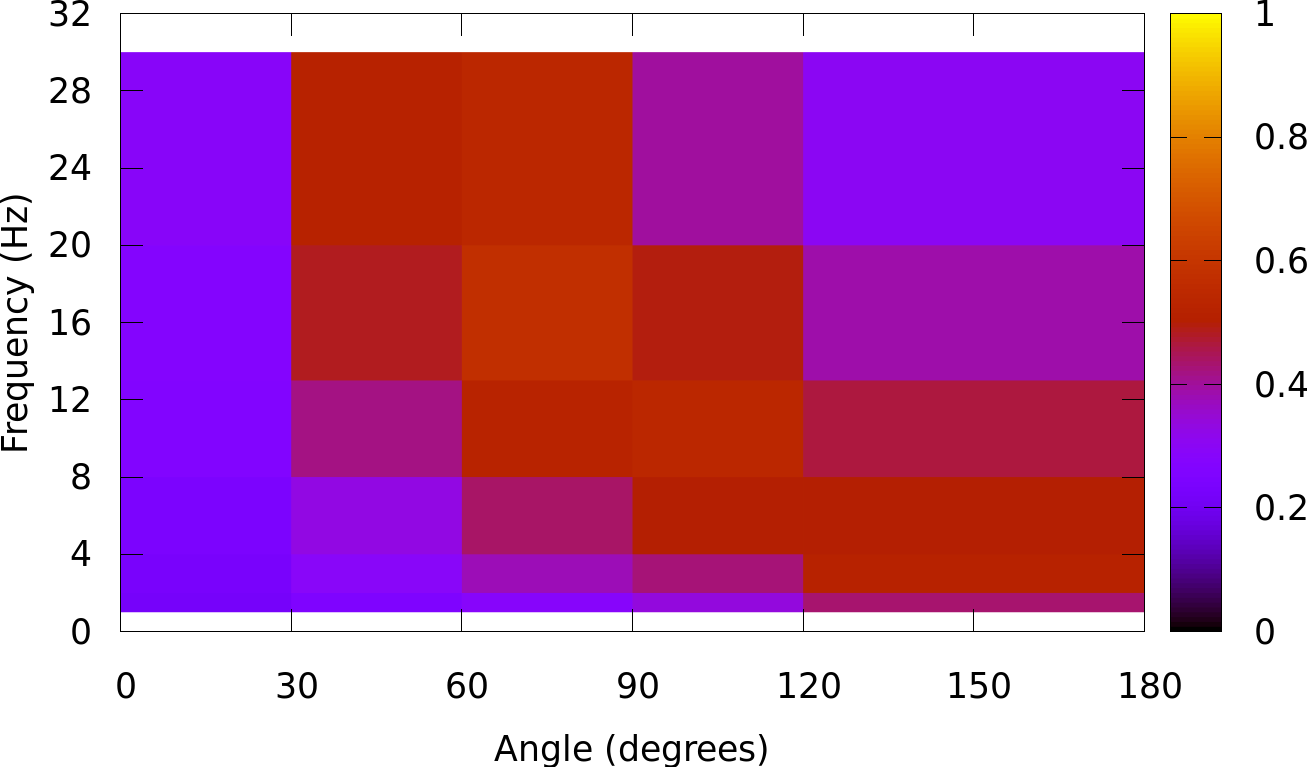
\includegraphics[width=\textwidth]{figures/ch4/average_times_081}
			\caption{MTSN pour $V = 2,19$.}
			\label{fig:hmap_t_219}
		\end{subfigure}
		~
		\begin{subfigure}[t]{\subImgWlineplot}
			\centering
			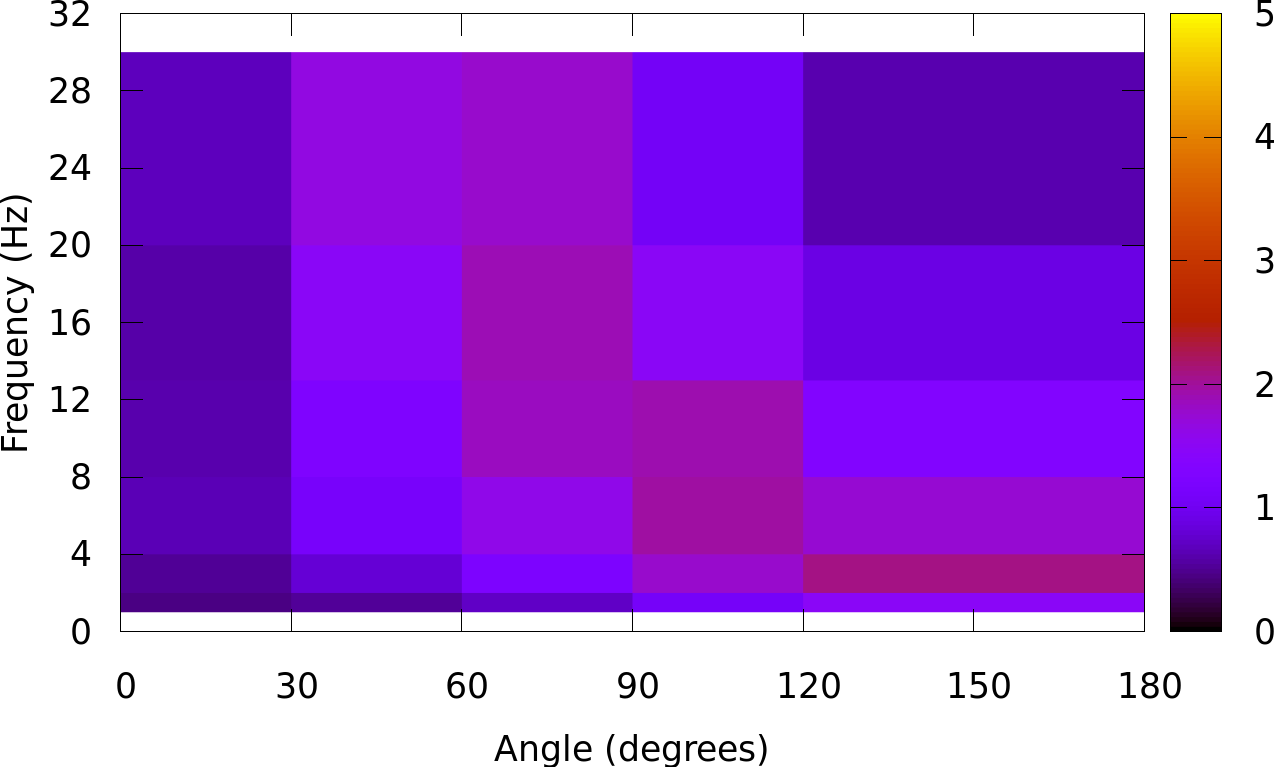
\includegraphics[width=\textwidth]{figures/ch4/average_error_rates_054}
			\caption{Taux d'erreurs pour $V = 1,46$.}
			\label{fig:hmap_e_146}
		\end{subfigure}
		~
		\begin{subfigure}[t]{\subImgWlineplot}
			\centering
			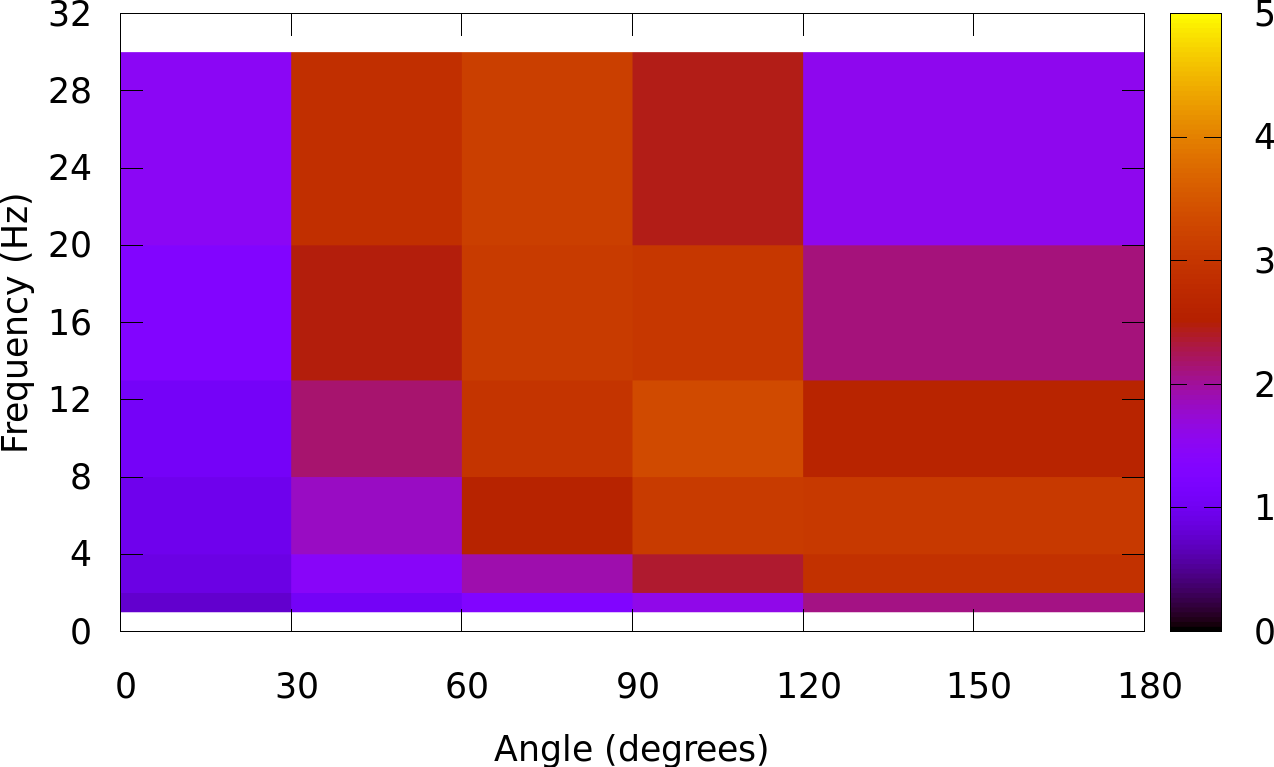
\includegraphics[width=\textwidth]{figures/ch4/average_error_rates_081}
			\caption{Taux d'erreurs pour $V = 2,19$.}
			\label{fig:hmap_e_219}
		\end{subfigure}
		~
		\begin{subfigure}[t]{\subImgWlineplot}
			\centering
			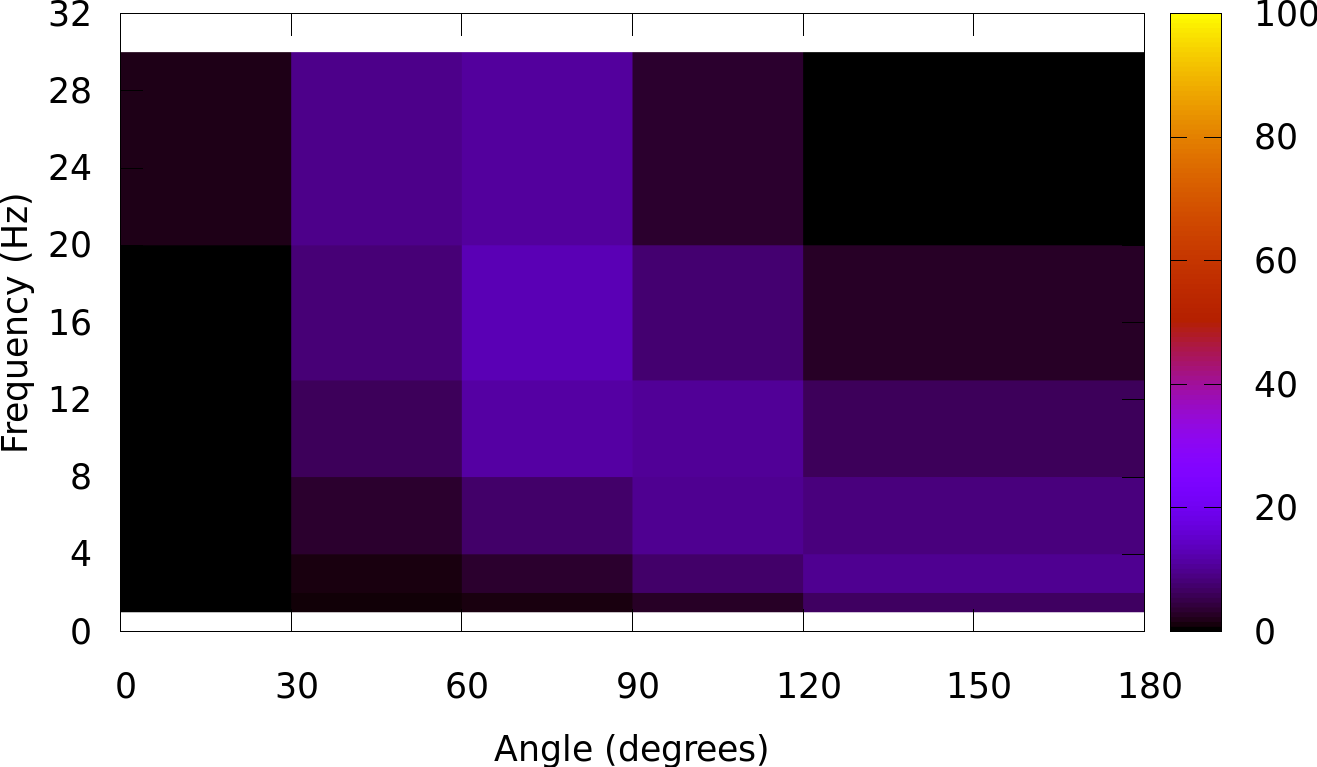
\includegraphics[width=\textwidth]{figures/ch4/average_failure_rates_054}
			\caption{Taux d'échecs pour $V = 2,19$.}
			\label{fig:hmap_f_146}
		\end{subfigure}
		~
		\begin{subfigure}[t]{\subImgWlineplot}
			\centering
			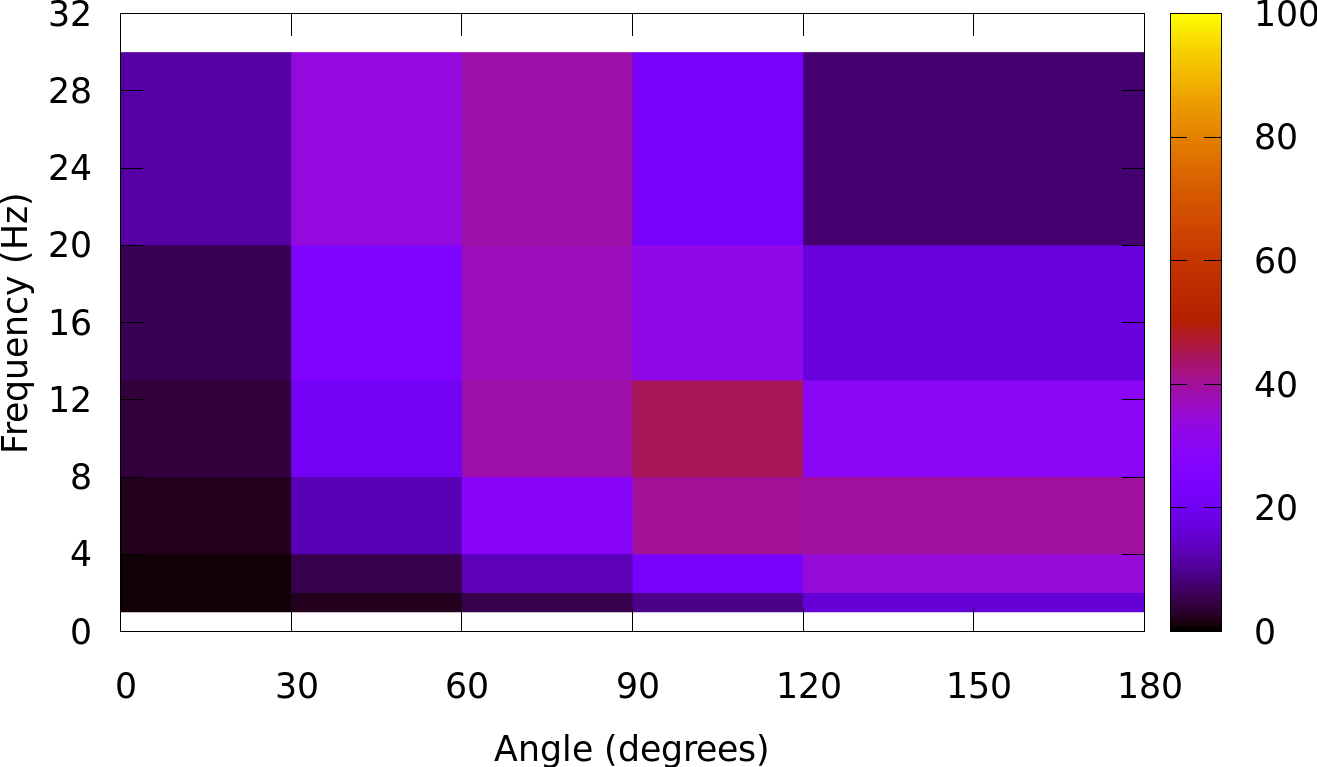
\includegraphics[width=\textwidth]{figures/ch4/average_failure_rates_081}
			\caption{Taux d'échecs pour $V = 2,19$.}
			\label{fig:hmap_f_219}
		\end{subfigure}
		\caption[Effets combinés de F et A sur les performances de sélection]{Effets combinés de F et A sur les performances de sélection. Les MTSN, TERR et TECH sont présentés pour toutes les valeurs de F et de A que nous avons testées, à moyenne et haute vitesse. Ces cartes thermiques (\emph{heat maps}) utilisent la couleur pour représenter une grandeur, selon l'échelle indiquée à leur droite. Les valeurs de A se lisent en abscisse, et celles de F en ordonnée. Ainsi, pour une vitesse données, toutes les combinaisons de A et F sont représentées.}
		\label{fig:hmaps}
	\end{figure}

	\subsection{Prévisibilité selon les angles et fréquences}
	Les tendances observées ci-dessus suggèrent que le produit de A et F (appelé pseudo-entropie dans le chapitre~\ref{chap3}) pourrait prédire les performances de sélection de cibles mobiles avec quelque efficacité. Nous avons tracé un graphique de la MTSN en fonction du produit AF, mettant en lumière les tendances observées pour A et F séparément, et leurs interactions, voir la figure~\ref{fig:tAF}.
	
	Plus spécifiquement, lorsque AF atteint une certaine valeur $AF_{pic}$ (ici située autour de 1100), le temps de sélection est maximal. Nous supposons que $AF_{pic}$ pourrait dépendre de plusieurs paramètres, tels que la largeur ou l'amplitude de Fitts, mais cette valeur est stable aux trois vitesses que nous avons évaluées, aussi en est-elle probablement indépendante. Naturellement, les tendances observées pour les MTSN valent également pour les TERR et TECH, très fortement corrélés aux MTSN (le coefficient de corrélation de Pearson entre les MTSN et TERR est supérieur à 0,959, avec une \emph{p-value} inférieure à $10^{-69}$).
	
	La figure~\ref{fig:tAF_Spnorm} présente $\frac{MTSN}{V}$, c'est-à-dire la MTSN normalisée par rapport à la vitesse, en fonction de AF. Les effets de AF étant trop faibles à basse vitesse, ils sont omis sur cette figure, et seules les vitesses moyenne et haute sont préservées.
	
	\begin{figure}[!htb]
		\begin{subfigure}[t]{0.49\textwidth}
			\centering
			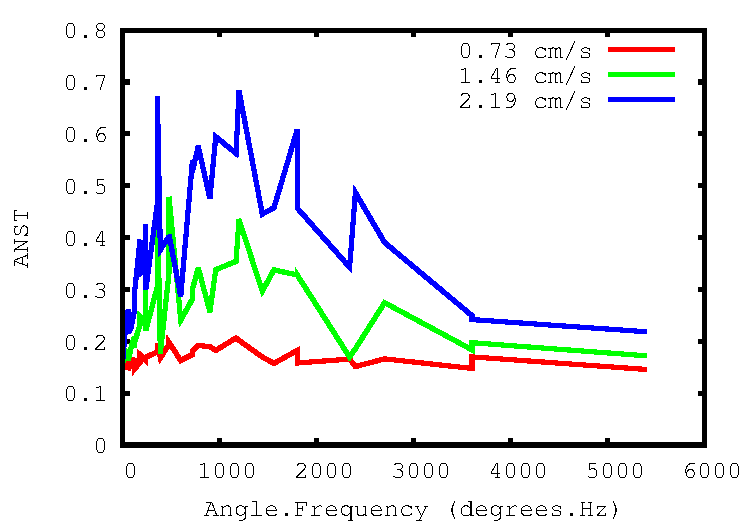
\includegraphics[width=\textwidth]{figures/ch4/time_vs_AF_all_speeds}
			\caption{MTSN en fonction du produit AF, pour chaque vitesse.}
			\label{fig:tAFallSp}
		\end{subfigure}
		~
		\begin{subfigure}[t]{0.49\textwidth}
			\centering
			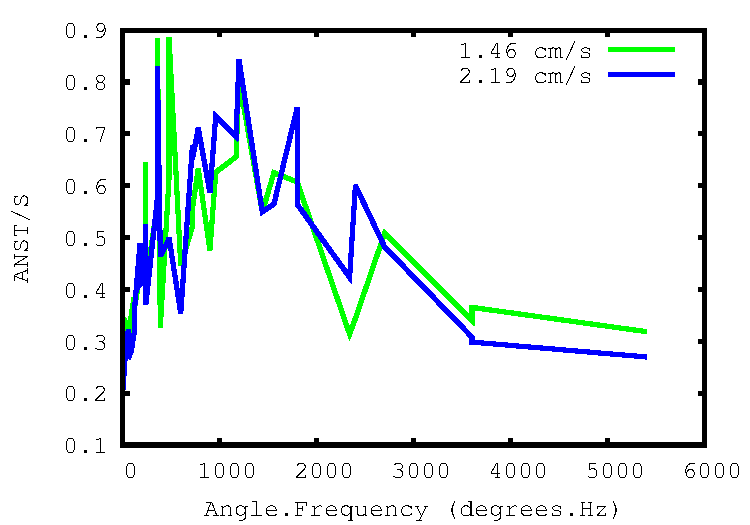
\includegraphics[width=\textwidth]{figures/ch4/time_vs_AF_all_speeds_normalized}
			\caption{$MTSN/V$ en fonction du produit AF, à moyenne et haute vitesse.}
			\label{fig:tAF_Spnorm}
		\end{subfigure}
		~
		\begin{subfigure}[t]{\textwidth}
			\centering
			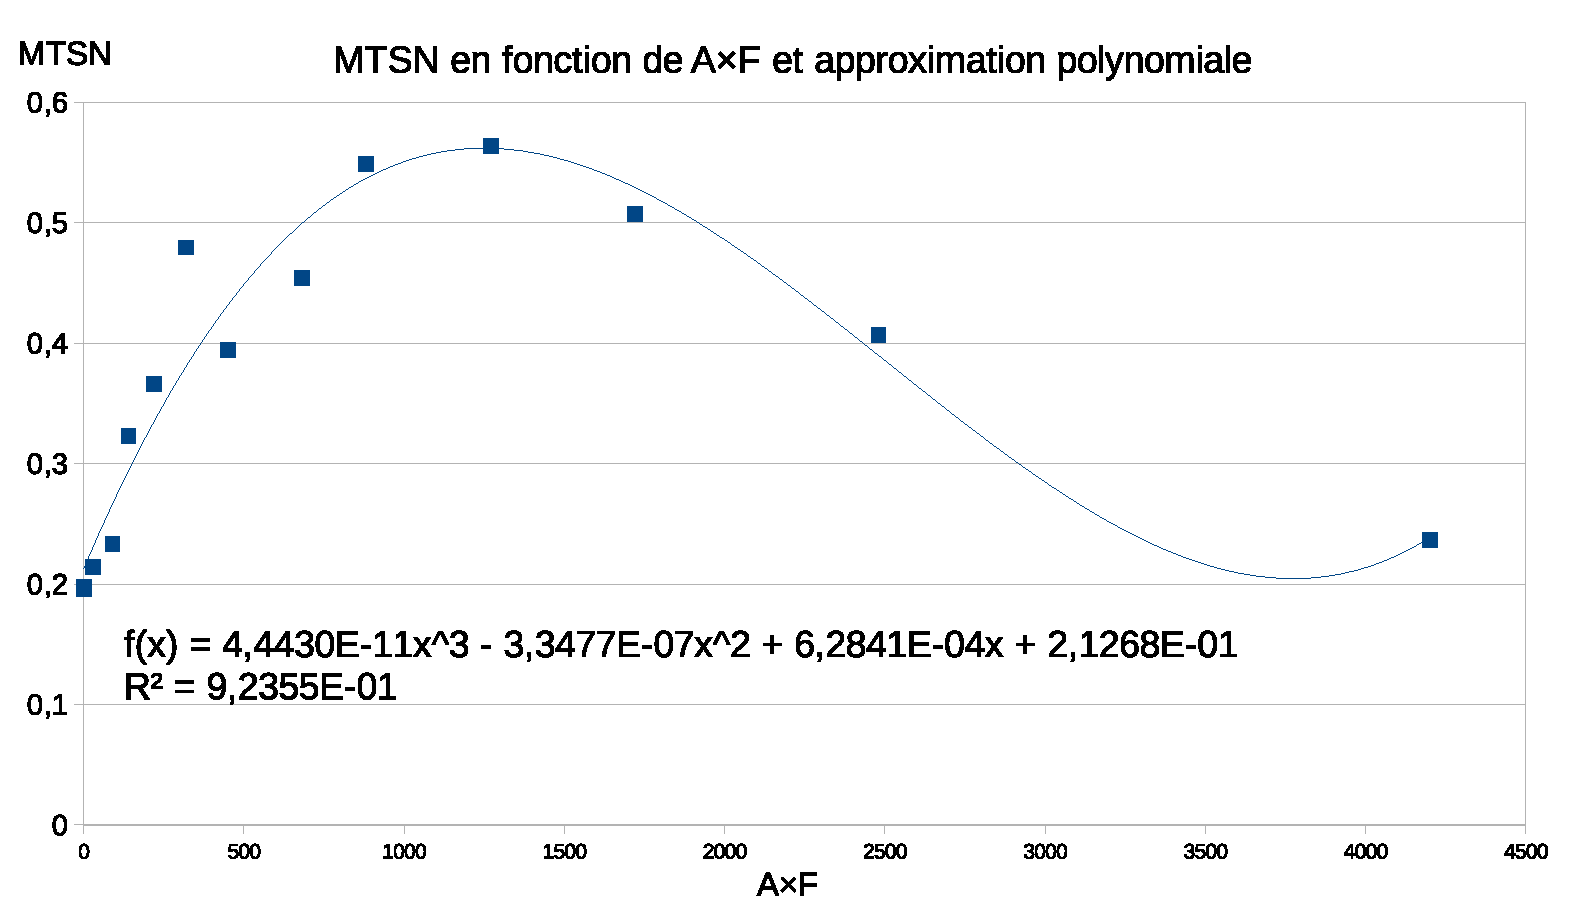
\includegraphics[width=\textwidth]{figures/ch4/MTSNvAF}
			\caption{MTSN sur les cibles rapides en fonction du produit AF après lissage, et approximation polynomiale (cubique). Le coefficient de détermination est légèrement supérieur à 92~\%{}, mais la croissance du polynome à partir de $AF \approx 3750$ montre bien que ce modèle ne peut être utile que sur un intervalle borné.}
			\label{fig:tAF_smooth}
		\end{subfigure}
		\caption[MTSN en fonction du produit AF]{MTSN en fonction du produit AF.}
		\label{fig:tAF}
	\end{figure}
	
	Comme on le constate, les courbes se superposent --- ce qui est assez logique compte tenu de l'effet approximativement linéaire de la vitesse sur les MTSN observé plus haut. Pour une vitesse donnée, la pseudo-entropie paraît donc offrir un moyen d'estimer la difficulté de sélection, par exemple en calculant la distance entre le produit AF d'une condition et la valeur $AF_{pic}$, si elle est connue.

	\subsection{Impressions subjectives}
	The answers to our questionnaire were consistent with, and complementary to, our quantitative results. Indeed, 92\%{} of our participants were able to identify different categories of motion: 77\%{} of them identified at least three major categories, together with two or three corresponding selection strategies.
Figure 3 - Selection time as a function of A×F. Screenshot of the application.

	\subsection{Catégories et stratégies}
	Participants first described rather steady motion, in roughly straight lines, with few or small deviations. In the second case, they identified “jerky” or “erratic” motion that they characterized by frequent, significant changes in direction. In the third case, they described the motion as “Brownian”, or “oscillations” or “vibrations”. More interestingly, 92\%{} of them explained that they would try to anticipate the target’s movement and to intercept it, and those who had identified a steady category specifically linked this strategy to it. However, our participants had no “clever” way of catching jerky targets, and would simply try to be fast enough and click a lot, thus making many errors. For the vibrating category, 69\%{} of them said
they would aim for the “average” position of the target over a short period of time, and either try to intercept it or just click and hope for the best.

	\subsection{Interprétation}
	The steady category reflects how our participants perceived the conditions where both angle width and change frequency were low. The jerky category relates to the difficult diagonal of our heat maps, and the vibrating category is the one with both high frequency and angle width. The important observation is that the strategy of anticipation requires a certain degree of predictability, since one can only anticipate what one can predict. Likewise, aiming for the average position of a target is a prediction. On the other hand, the jerky category seems to be very difficult to predict. We therefore conclude that the steady and vibrating categories of moving targets are relatively easy to acquire because their movements are quite predictable, whereas jerky targets are more difficult because less predictable. Of course, the borders between these categories are hard to determine formally and are likely to depend on the user perception of the movement.

\section{Conclusion and perspectives}
We have proposed a way to characterize the erratic behavior of moving targets with three parameters: speed, angle width and frequency, and tested pointing performance when varying these parameters. We have shown that the nature of target motion affects pointing performance, which is not captured by Fitts’ law’s index of difficulty. The latter can only describe the best case, and does not indicate that acquiring fast, highly erratic targets can be extremely difficult. Although the (S,A,F) set of parameters we have proposed models a continuum of target motion, our participants were able to distinguish at least three distinct categories that we have characterized (steady, vibrating and jerky). Our results suggest that
for erratic targets, predictability determines pointing performance. And while the steady and vibrating categories are relatively predictable, the jerky one is not. We have also observed that the A×F product might be a promising way to assess predictability, although we still need more data to deduce a predictive law for the acquisition of erratic targets. Nevertheless, this preliminary work is a first step toward a more formal study of the acquisition of erratic targets, and introduces a way to better characterize or even control their movement. Ultimately, such a model could be
instrumental in the design of new selection techniques.

\clearpage
